\let\negmedspace\undefined
\let\negthickspace\undefined
\documentclass[journal]{IEEEtran}
\usepackage[a5paper, margin=10mm, onecolumn]{geometry}
%\usepackage{lmodern} % Ensure lmodern is loaded for pdflatex
\usepackage{tfrupee} % Include tfrupee package

\setlength{\headheight}{1cm} % Set the height of the header box
\setlength{\headsep}{0mm}     % Set the distance between the header box and the top of the text

\usepackage{gvv-book}
\usepackage{gvv}
\usepackage{cite}
\usepackage{amsmath,amssymb,amsfonts,amsthm}
\usepackage{algorithmic}
\usepackage{graphicx}
\usepackage{textcomp}
\usepackage{xcolor}
\usepackage{txfonts}
\usepackage{listings}
\usepackage{enumitem}
\usepackage{mathtools}
\usepackage{gensymb}
\usepackage{comment}
\usepackage[breaklinks=true]{hyperref}
\usepackage{tkz-euclide} 
\usepackage{listings}
\usepackage{gvv}                                        
\def\inputGnumericTable{}                                 
\usepackage[latin1]{inputenc}                                
\usepackage{color}                                            
\usepackage{array}                                            
\usepackage{longtable}                                       
\usepackage{calc}                                             
\usepackage{multirow}                                         
\usepackage{hhline}                                           
\usepackage{ifthen}                                           
\usepackage{lscape}
\begin{document}

\bibliographystyle{IEEEtran}

\title{8.4.22}
\author{EE25BTECH11019 - Darji Vivek M.}
{\let\newpage\relax\maketitle}

\renewcommand{\thefigure}{\theenumi}
\renewcommand{\thetable}{\theenumi}
\setlength{\intextsep}{10pt}
\numberwithin{figure}{enumi}
\renewcommand{\thetable}{\theenumi}

\textbf{Question:}\\[2pt]
The radius of the circle passing through the foci of the ellipse
\[
\frac{x^2}{16}+\frac{y^2}{9}=1
\]
and having its centre at $(0,3)$ is -\\[6pt]
\begin{multicols}{4}
\begin{enumerate}
    \item $4$
    \item $3$
    \item $\sqrt{\frac{1}{2}}$
    \item $\frac{7}{2}$
\end{enumerate}
\end{multicols}

\solution\\[-2mm]

\solution\\[4pt]
Let \(\vec x=\myvec{x\\[2pt]y}\). The given ellipse is
\[
\frac{x^2}{16}+\frac{y^2}{9}=1
\qquad\Longleftrightarrow\qquad
\vec x^\top\vec V\vec x=1,\qquad
\vec V=\myvec{\frac{1}{16} & 0\\[2pt]0 & \frac{1}{9}}.
\]

The eigenvalues (principal values) of \(\vec V\) are its diagonal entries; take them in increasing order
\[
\lambda_1=\frac{1}{16},\qquad \lambda_2=\frac{1}{9}.
\]
Hence the squared semi-axes (principal-form relations) are
\[
a^2=\frac{1}{\lambda_1}=16,\qquad b^2=\frac{1}{\lambda_2}=9,
\]
so \(a=4,\ b=3\).

Using the formula for eccentricity.
\[
e=\sqrt{1-\frac{\lambda_1}{\lambda_2}}
=\sqrt{1-\frac{1/16}{1/9}}
=\sqrt{1-\frac{9}{16}}
=\sqrt{\frac{7}{16}}
=\frac{\sqrt7}{4}.
\]
The focal distance (from the centre) is \(c = a e\), therefore
\[
c = 4\cdot\frac{\sqrt7}{4}=\sqrt7.
\]
Since \(\vec V\) is diagonal with \(\lambda_1\) along the x-direction, the principal axis unit vector is.

\[
\vec n=\myvec{1\\[2pt]0}.
\]
Thus the foci (in vector form) are
\[
\vec F_1 = c\vec n = \myvec{\sqrt7\\[2pt]0},\qquad
\vec F_2 = -c\vec n = \myvec{-\sqrt7\\[2pt]0}.
\]

The required circle has centre \(C=\myvec{0\\[2pt]3}\) and passes through either focus, so the radius is
\[
R=\norm{\vec F_1-\vec C}
=\sqrt{(\sqrt7-0)^2+(0-3)^2}
=\sqrt{7+9}
=\sqrt{16}=4.
\]

Therefore the radius of the required circle is
\(
\boxed{4}.
\)


 \begin{figure}[H]
     \centering
     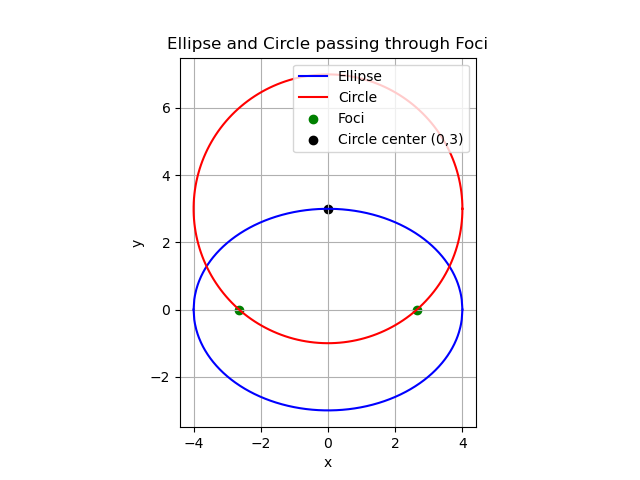
\includegraphics[width=0.8\columnwidth]{figs/15.png}
     \label{fig:1}
 \end{figure}

\end{document}
Use the matrix form (matrix method). Let $\vec{x}=\myvec{x\\[2pt]y}$. The ellipse is
\[
\vec{x}^\top \vec{V}\,\vec{x}=1,\qquad
\vec{V}=\myvec{\frac{1}{16} & 0\\[2pt]0 & \frac{1}{9}}.
\]
Eigenvalues of $\vec{V}$ (diagonal entries) are
\[
\lambda_1=\frac{1}{16},\qquad \lambda_2=\frac{1}{9}.
\]
For the principal-form ellipse $\vec{x}^\top\vec{V}\vec{x}=1$ the semi-axes satisfy
\[
a^2=\frac{1}{\lambda_1}=16,\qquad b^2=\frac{1}{\lambda_2}=9.
\]
Hence the focal distance from origin is
\[
c=\sqrt{a^2-b^2}=\sqrt{16-9}=\sqrt{7}.
\]
Thus the foci (in matrix/vector form) are
\[
F_1=\myvec{\sqrt{7}\\[2pt]0},\qquad F_2=\myvec{-\sqrt{7}\\[2pt]0}.
\]
The required circle has centre $C=\myvec{0\\[2pt]3}$ and passes through, say, $F_1$. Therefore its radius is
\[
R=\norm{F_1-C}
=\sqrt{\bigl(\sqrt{7}-0\bigr)^2+\bigl(0-3\bigr)^2}
=\sqrt{7+9}
=\sqrt{16}
=\boxed{4}.
\]